\chapter{Code}

\section*{Source Code Repository}
The complete source code for the MARVIS system, including the YOLOv8 fine-tuning scripts, DeepOCSORT integration, LSTM trajectory predictor, and the real-time WebSocket dashboard, is available on GitHub at:
\begin{center}
    \url{https://github.com/ShashankShenoy/Major_Project}
\end{center}


\section{System Dashboard Interfaces}
The following figures illustrate the MARVIS web dashboard and annotated video outputs, which serve as the primary operator interfaces for the maritime surveillance system.

\begin{figure}[H]
\centering
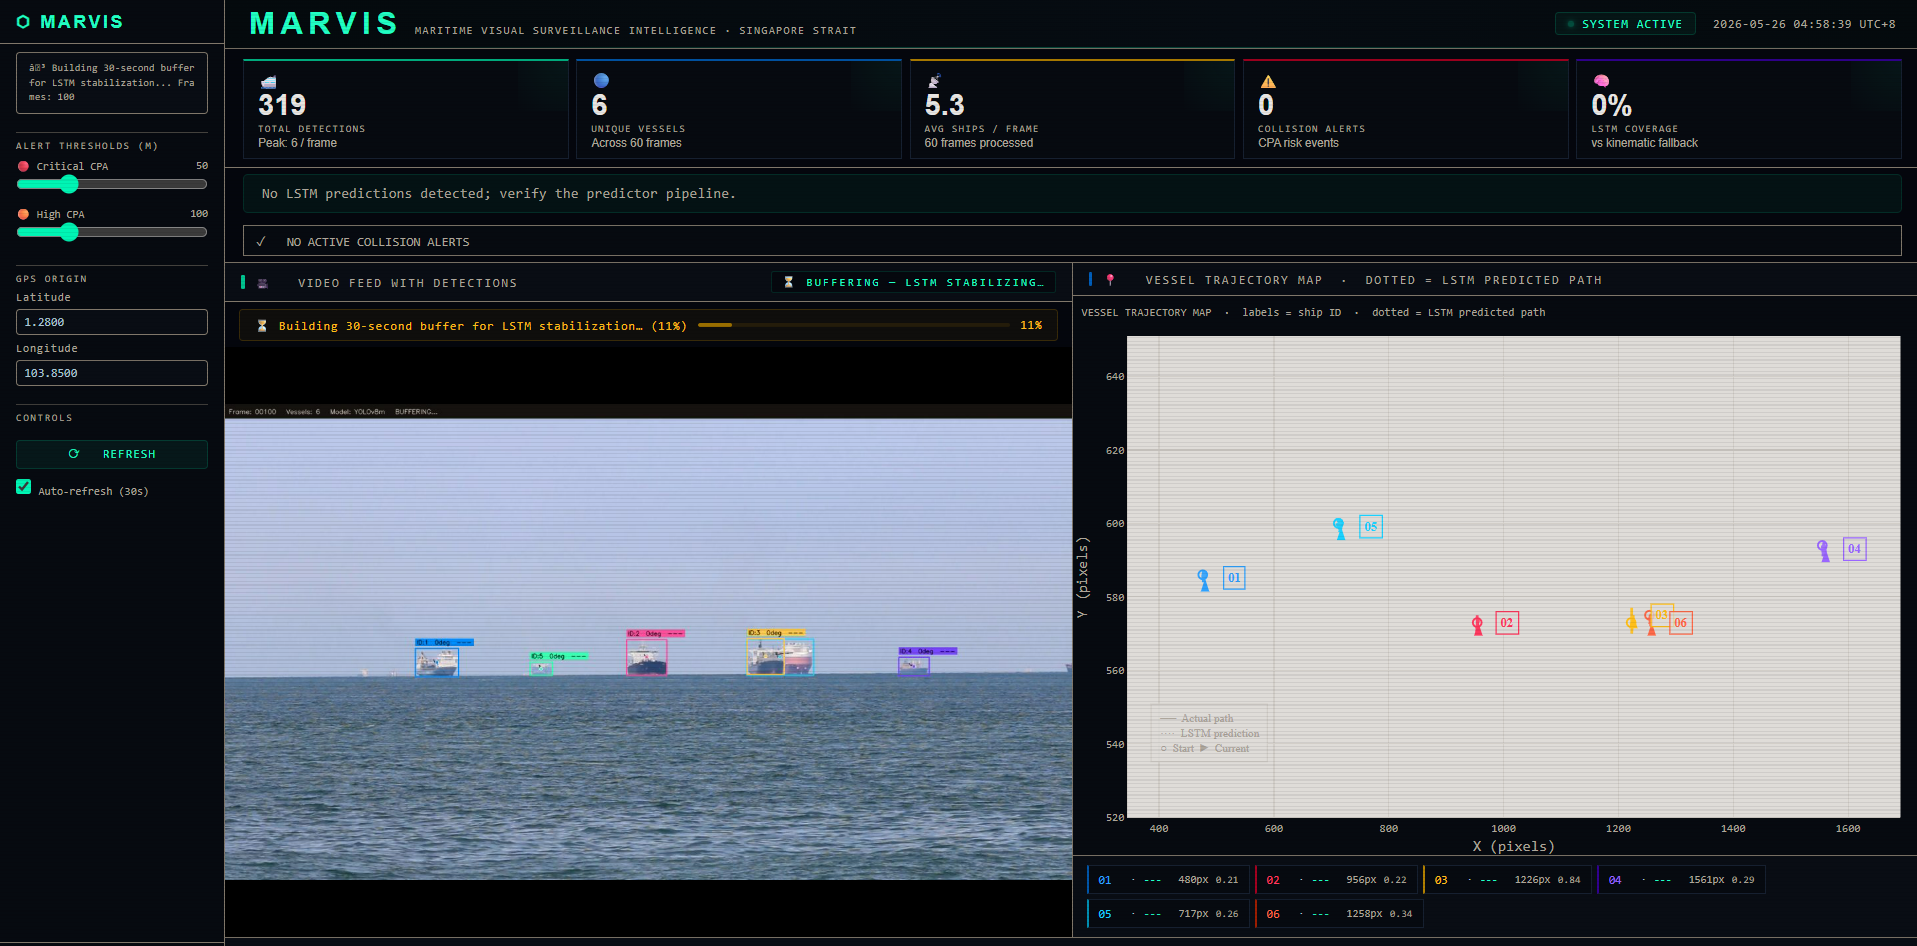
\includegraphics[width=0.95\textwidth]{Chapter5/Figures/dashboard_full.png}
\caption{MARVIS Primary Dashboard Interface showing telemetry, video feed, and real-time mapping.}
\end{figure}

\begin{figure}[H]
\centering
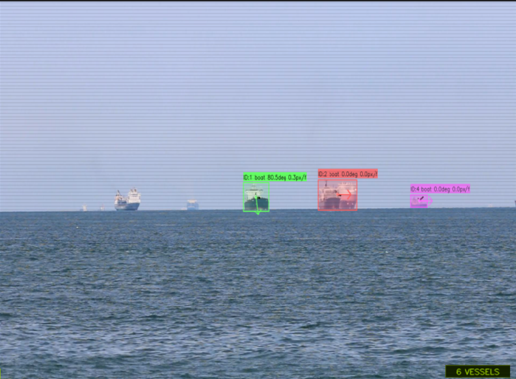
\includegraphics[width=0.95\textwidth]{Chapter5/Figures/detection_output.png}
\caption{Real-time Annotated Video Feed with bounding boxes.}
\end{figure}

\begin{figure}[H]
\centering
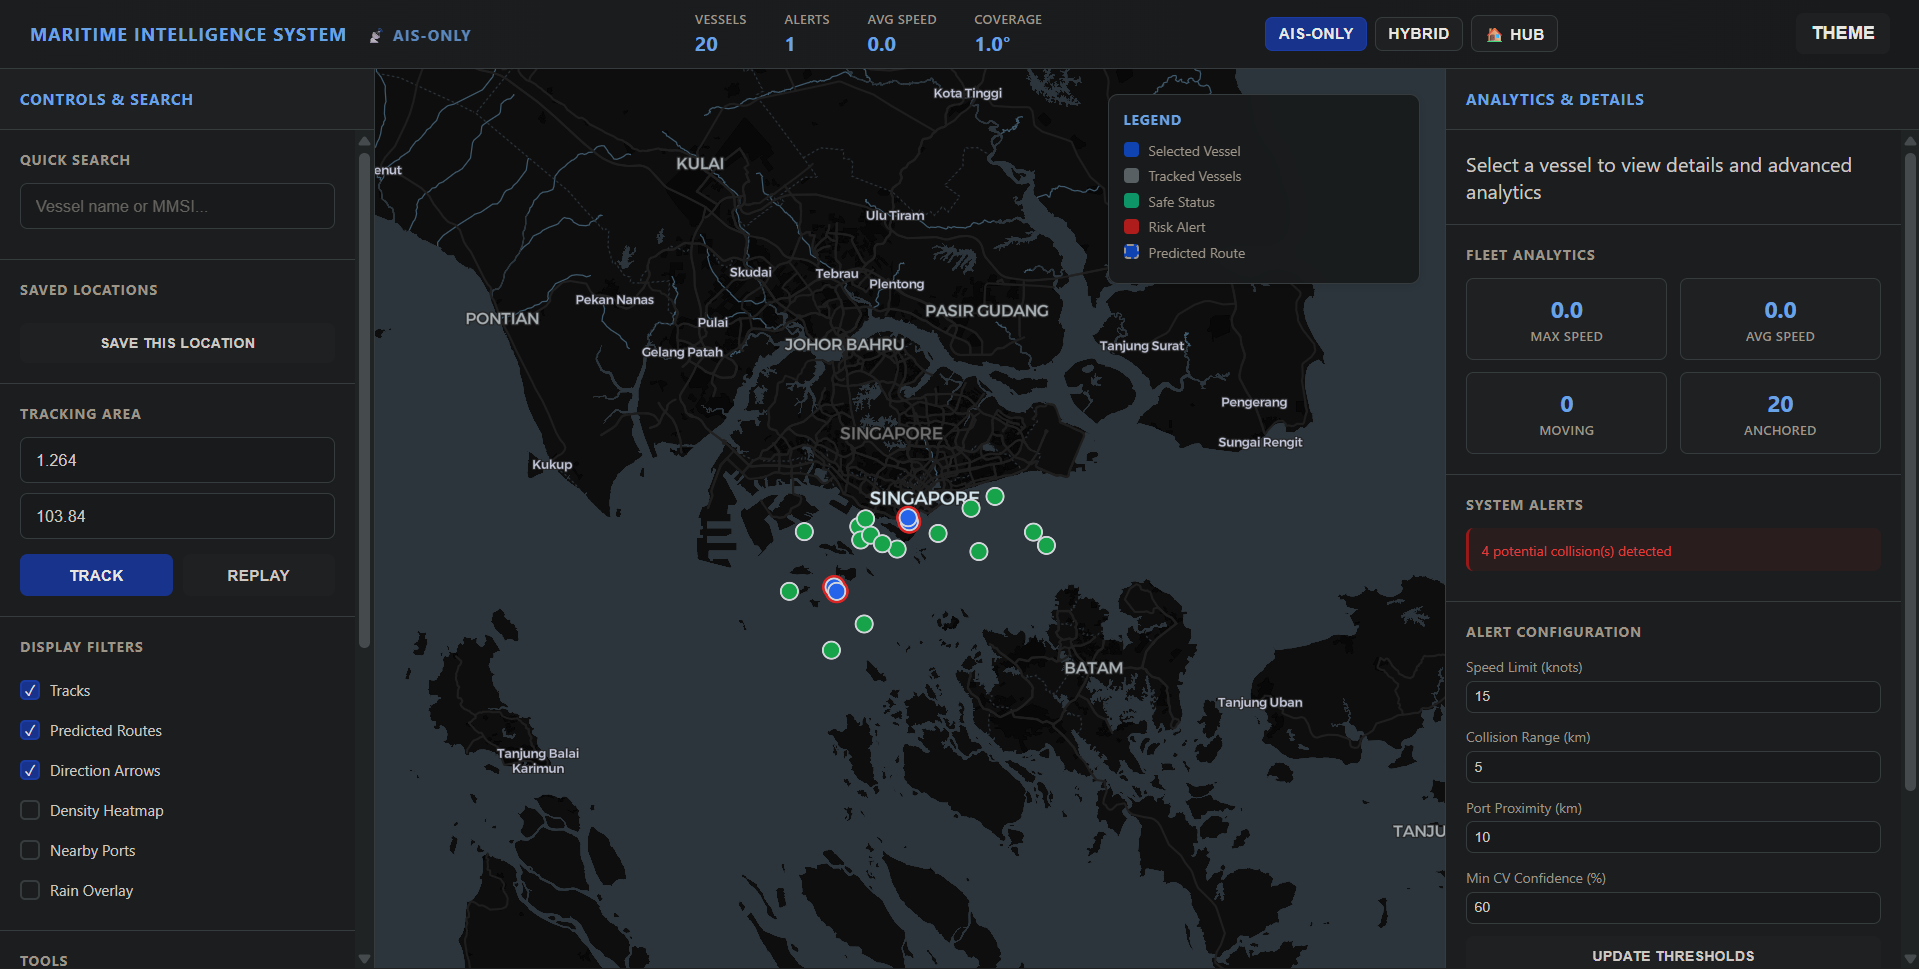
\includegraphics[width=0.95\textwidth]{Chapter5/Figures/ais_fusion_map.png}
\caption{Geospatial AIS Sensor Fusion Map indicating cooperative vessels and potential dark traffic.}
\end{figure}


\section{AIS-Matched Vessel Inference Routing}
The following snippet from \texttt{cv\_matcher.py} illustrates the CV-to-AIS matching logic, which enables the LSTM skip optimization for cooperative vessels.

\begin{tcblisting}{listing only,colback=gray!10!white, breakable, boxsep=0pt,top=1mm,bottom=1mm,left=1mm,right=1mm,
listing options={
language=python,
basicstyle=\small\ttfamily, 
keywordstyle=\color{blue}, 
commentstyle=\color{gray},
backgroundcolor=\color{gray!25},
showspaces=false,
showstringspaces=false,
columns=fullflexible,
escapechar=!}}
def match_cv_to_ais(
    cv_detection: ShipDetection,
    ais_ships: Dict[int, Dict],
    match_radius_km: float = 5.5
) -> Optional[Tuple[int, float]]:
    """Match a camera detection to an AIS ship within a threshold radius."""
    best_match = None
    best_distance = match_radius_km

    for mmsi, ais_ship in ais_ships.items():
        if not ais_ship.get("history") or len(ais_ship["history"]) < 1:
            continue
        
        # Get latest AIS position
        latest_pos = ais_ship["history"][-1]
        distance = calculate_distance_km(
            (cv_detection.gps_lat, cv_detection.gps_lon),
            (latest_pos[1], latest_pos[2])
        )
        
        # Update best match if closer
        if distance < best_distance:
            best_distance = distance
            best_match = (mmsi, distance)
            
    return best_match

def enrich_cv_detection_with_ais(
    cv_detection: ShipDetection, 
    ais_ship: Dict
) -> ShipDetection:
    """Enrich a CV detection with AIS data to skip LSTM prediction."""
    cv_detection.is_matched_to_ais = True
    cv_detection.matched_ais_mmsi = ais_ship.get("mmsi")
    
    # Update with AIS motion data if available
    if "sog" in ais_ship:
        cv_detection.sog = ais_ship["sog"]
    if "cog" in ais_ship: 
        cv_detection.cog = ais_ship["cog"]
        cv_detection.heading = ais_ship["cog"]
        
    return cv_detection
\end{tcblisting}

\section{Dashboard Pipeline Integration Loop}
The following snippet from \texttt{marvis\_api.py} demonstrates the core frame-processing loop where YOLOv8 detection, DeepOCSORT tracking, and LSTM trajectory prediction are integrated into a single real-time pipeline.

\begin{tcblisting}{listing only,colback=gray!10!white, breakable, boxsep=0pt,top=1mm,bottom=1mm,left=1mm,right=1mm,
listing options={
language=python,
basicstyle=\small\ttfamily, 
keywordstyle=\color{blue}, 
commentstyle=\color{gray},
backgroundcolor=\color{gray!25},
showspaces=false,
showstringspaces=false,
columns=fullflexible,
escapechar=!}}
# YOLO detection 
try:
    det_results = yolo_model(
        frame,
        conf    = CONFIDENCE,
        classes = CLASSES,
        verbose = False
    )[0]
    dets = det_results.boxes.data.cpu().numpy()
except Exception as e:
    dets = np.empty((0, 6))

# DeepOcSort tracking
try:
    if len(dets) > 0:
        tracks = tracker.update(dets, frame)
    else:
        tracks = tracker.update(np.empty((0, 6)), frame)
except Exception as e:
    tracks = []

# Build ship list and Predict
for t in (tracks if tracks is not None and len(tracks) > 0 else []):
    try:
        x1, y1, x2, y2 = int(t[0]), int(t[1]), int(t[2]), int(t[3])
        sid            = int(t[4])

        cx = (x1 + x2) // 2
        cy = (y1 + y2) // 2
        history[sid].append((cx, cy))

        smoothed = smooth_history(history[sid])

        # LSTM / kinematic prediction
        if buffer_complete and frame_count % update_frame_interval == 0:
            if lstm_engine:
                lstm_engine.update(str(sid), cx, cy)
                pred, method = lstm_engine.predict(str(sid))
                persistent_predictions[sid] = pred
            else:
                persistent_predictions[sid] = predict_kinematic(smoothed)
        
        predicted_path = persistent_predictions.get(sid, [])
        
    except Exception as e:
        continue
\end{tcblisting}